\chapter{PPO mit bedingtem Aktionsraum}
\label{ch:ppo_bedingt}

Standard \ac{RL}\hyp{}Algorithmen basieren üblicherweise auf der Annahme, dass Aktionen stochastisch unabhängig voneinander sind.
Im hier betrachteten Szenario ist diese Annahme jedoch verletzt, da die kontinuierliche Komponente des gemischten Aktionsraums nur dann relevant ist, wenn sich der Agent für eine \emph{Heading}\hyp{}Änderung entscheidet.
In Fällen, in denen \emph{Noop} oder \emph{Direct Route} gewählt wird, hat der Wert der kontinuierlichen Aktion keinen Einfluss auf die Umgebung.
Dennoch würde der Standard\hyp{}PPO\hyp{}Algorithmus Gradienten für diese irrelevante Komponente berechnen. Dies führt zu Fehloptimierungen, da der Agent Ressourcen darauf verwendet, eine in diesem Kontext wirkungslose Aktion zu optimieren, was das Lernen der relevanten Strategien behindert.
\vspace{\baselineskip}

Um dieses Problem zu adressieren, wurde ein aktionsabhängiges Gradient\hyp{}Gating implementiert, welches die Rückpropagation von Gradienten für irrelevante Aktionen unterbindet.

\section{Gradient\hyp{}Gating im PPO\hyp{}Algorithmus}
\label{sc:ppo_anpassung}

Der gewählte Lösungsansatz weist Parallelen zu dem in \cite{invalid_Action_Masking} vorgestellten \emph{Invalid Action Masking} auf. Dort wird ein zustandsabhängiges Gating verwendet, um ungültige Aktionen bereits während der Rollout\hyp{}Phase zu maskieren.
Dieser Ansatz ist für das vorliegende Problem jedoch nicht direkt übertragbar, da die Relevanz der kontinuierlichen Aktion nicht allein vom Zustand, sondern von der im gleichen Schritt gesampelten diskreten Aktion abhängt. Da zum Zeitpunkt des Maskierens im Rollout die Aktion noch nicht feststeht, ist ein solches präemptives Gating nicht möglich.
\vspace{\baselineskip}

Stattdessen wird in dieser Arbeit ein Gradient\hyp{}Gating implementiert. Dabei werden alle Aktionen zunächst gesampelt, jedoch wird die Gradientenberechnung für die kontinuierliche Aktion nachträglich unterdrückt, falls diese sich als irrelevant erweist. Die maskierte Ausführung in der Umgebung stellt dabei sicher, dass irrelevante Aktionen auch tatsächlich keine Zustandsänderung bewirken.
\vspace{\baselineskip}

Die technische Umsetzung erfolgt durch gezielte Anpassungen der SB3\hyp{}Plus Bibliothek \cite{sb3_plus}. Die vollständigen Änderungen an der Implementierung sind im Anhang in Abschnitt \ref{sc:ppo_code} zu finden.
Das Verfahren greift in drei zentrale Komponenten des PPO\hyp{}Algorithmus ein, deren theoretische Fundierung in Abschnitt \ref{ch:rl_grundlagen} erläutert wurde.

Da der Policy\hyp{}Loss $L_t^{CLIP}$ (siehe Gleichung \ref{eq:clip_loss}) über das Wahrscheinlichkeitsverhältnis $r_t(\theta)$ direkt von den logarithmischen Wahrscheinlichkeiten der Aktionen abhängt, ist an dieser Stelle ein Eingriff notwendig, um den Einfluss irrelevanter Aktionskomponenten auf den Gradienten zu eliminieren. Analog muss der Entropie\hyp{}Term $S[\pi_\theta]$ angepasst werden, um eine Belohnung für die Variation wirkungsloser Aktionen zu verhindern. Der Term der Wertfunktion $L_t^{VF}(\phi)$ (siehe Gleichung \ref{eq:value_loss}) hingegen bleibt von diesen Modifikationen unberührt, da der Critic $V_\phi(s_t)$ den Wert eines Zustandes unabhängig von der spezifischen Struktur des im gleichen Zeitschritt gewählten Aktionsvektors schätzt.

Die konkrete technische Umsetzung dieser theoretischen Überlegungen erfordert Eingriffe an drei Stellen der Implementierung: der Definition der Wahrscheinlichkeitsverteilung, der Evaluationsmethode für das Training und dem Vorwärtsschritt für die Datensammlung. Im Folgenden werden diese Anpassungen im Detail beschrieben.

\subsection*{Wahrscheinlichkeitsverteilung}
Die Klasse der Wahrscheinlichkeitsverteilung wurde erweitert, um logarithmische Wahrscheinlichkeiten (\texttt{log\_prob()}) und Entropien (\texttt{entropy()}) getrennt für diskrete und kontinuierliche Aktionen auszuwerten. Während die Basisimplementierung diese Werte sofort summiert, ermöglicht die Modifikation den Zugriff auf separierte Tensoren. Dies ist die Voraussetzung, um im nächsten Schritt eine selektive Maskierung vornehmen zu können.

\subsection*{Evaluation}
In der Methode \texttt{evaluate\_actions()}, welche während der Optimierungsphase aufgerufen wird (siehe Algorithmus \ref{alg:ppo_training}, Zeile 20), werden die Komponenten der PPO\hyp{}Verlustfunktion berechnet. Hier erfolgt das eigentliche Gradient\hyp{}Gating.
Mithilfe einer binären Maske wird sichergestellt, dass die kontinuierliche Verteilung nur dann Einfluss auf die Gradientenbildung hat, wenn sie entscheidungsrelevant ist.
Algorithmus \ref{alg:gradient_gating} zeigt die Implementierung dieser Logik.

\begin{algorithm}
\caption{Gradient-Gating in der Evaluationsfunktion}
\label{alg:gradient_gating}
\begin{algorithmic}[1]
\State \texttt{mask = (actions[:, 0] == STEER\_INDEX).bool()}
\Statex
\State \texttt{log\_prob = dist.stack\_log\_prob(actions)}
\State \texttt{action\_type\_log\_prob = log\_prob[:, 0]}
\State \texttt{steer\_log\_prob = log\_prob[:, 1]}
\Statex
\State \texttt{steer\_log\_prob = th.where(mask, steer\_log\_prob,}
\Statex \qquad \qquad \qquad \qquad \qquad \qquad \texttt{th.zeros\_like(steer\_log\_prob))}
\State \texttt{masked\_log\_prob = action\_type\_log\_prob + steer\_log\_prob}
\Statex
\State \texttt{with th.no\_grad():}
\State \quad \texttt{steer\_distribution = dist.distribution[0].distribution}
\State \quad \texttt{p\_steer = steer\_distribution.probs[:, STEER\_INDEX]}
\Statex
\State \texttt{entropy = dist.stack\_entropy()}
\State \texttt{action\_type\_entropy = entropy[:, 0]}
\State \texttt{steer\_entropy = entropy[:, 1]}
\Statex
\State \texttt{masked\_entropy = action\_type\_entropy + p\_steer * steer\_entropy}
\end{algorithmic}
\end{algorithm}
\vspace{\baselineskip}

In Zeile 5 wird für die logarithmischen Wahrscheinlichkeiten eine explizite Null\hyp{}Maskierung vorgenommen.
Der Aufruf \texttt{th.zeros\_like()} erzeugt dabei einen neuen Tensor, der standardmäßig nicht Teil des Berechnungsgraphen ist (\texttt{requires\_grad=False}).
Dies stellt technisch sicher, dass für die maskierten Einträge keine Gradienten zurückfließen.
Mathematisch bedeutet dies, dass die irrelevante kontinuierliche Aktion als deterministisch betrachtet wird (Wahrscheinlichkeit 1, $\log(1)=0$) und somit keinen Beitrag zur Gesamt\hyp{}Log\hyp{}Likelihood leistet.
Auf diese Weise wird verhindert, dass irrelevante Aktionen die Update\hyp{}Schritte des PPO verfälschen.
\vspace{\baselineskip}

Für die Regularisierung durch Entropie (Zeile 12) wird das Konzept der bedingten Entropie umgesetzt. Die Gesamtentropie berechnet sich als Summe der diskreten Entropie und der mit ihrer Auftrittswahrscheinlichkeit gewichteten kontinuierlichen Entropie:
\begin{equation}
    H_{\text{total}} = H(a_{\text{type}}) + p(a_{\text{type}}=\text{Steer}) \cdot H(a_{\text{steer}})
\end{equation}

Ein entscheidendes Detail zur Vermeidung von Fehloptimierungen (Bias) ist die Behandlung des Gewichtungsfaktors $p(\text{Steer})$ in Zeile 8. Dieser wird innerhalb eines \texttt{no\_grad}\hyp{}Blocks extrahiert und somit vom Gradientenfluss entkoppelt.
Würde man $p(\text{Steer})$ direkt verwenden, würde der Agent lernen, die Wahrscheinlichkeit für die \emph{Steer}\hyp{}Aktion allein deshalb zu erhöhen, um den additiven Entropie\hyp{}Term zu maximieren.
Durch die Verwendung von \texttt{no\_grad()} wirkt die Wahrscheinlichkeit lediglich als konstanter Skalierungsfaktor für die kontinuierliche Entropie, wodurch dieser Bias eliminiert wird.

\subsection*{Vorwärtsschritt}
Analog zur Evaluation muss das Gradient\hyp{}Gating auch im Vorwärtsschritt angewendet werden. Die \texttt{forward()}\hyp{}Funktion wird während der Rollout\hyp{}Phase durchlaufen (siehe Algorithmus \ref{alg:ppo_training}, Zeile 7). Die logarithmischen Wahrscheinlichkeiten werden hier ebenfalls null\hyp{}maskiert, bevor sie im Rollout\hyp{}Buffer gespeichert werden. Dies gewährleistet, dass die gespeicherten Referenzwerte ($\pi_{\text{old}}$) konsistent zu den im Training neu berechneten Werten sind und die \emph{Probability Ratios} korrekt gebildet werden können.

\section{Herausforderungen in bedingten Aktionsräumen}

Die Verwendung bedingter Aktionsräume stellt das Training von Reinforcement-Learning-Agenten vor spezifische Herausforderungen, die über rein technische Implementierungsdetails hinausgehen. Ein zentrales Problem ergibt sich aus der Kopplung von Aktionen und der daraus resultierenden Häufigkeit von Feedback Signalen für die einzelnen Aktionskomponenten. Wenn relevante Aktionen aufgrund der hierarchischen Struktur nur selten ausgeführt werden, kann dies den Lernprozess erheblich beeinträchtigen.

\subsection*{Sparsity-Problematik der abhängigen Aktion}
In der frühen Trainingsphase neigen Agenten oft dazu, initial suboptimale Strategien zu verfolgen. Wählt der Agent überwiegend Aktionen, die abhängigen Aktion blockieren (z.\,B. \emph{Noop}), erhält das Netzwerk für die abhängige Aktion (\emph{Steer}) kaum Gradienteninformationen. Ein unoptimierter Steer-Wert führt bei seiner seltenen Ausführung häufig zu negativem Feedback, was den Agenten wiederum dazu verleitet, die Nutzung dieser Aktion weiter zu vermeiden. Dieser Rückkopplungseffekt kann dazu führen, dass die Wahrscheinlichkeitsverteilung für die Aktivierung der kontinuierlichen Komponente gegen Null geht, bevor der Agent genügend Erfahrungen sammeln konnte, um eine effektive Lenkstrategie zu erlernen.

\subsection*{Destruktive Interferenz und Lokale Optima}
Szenarien, in denen die übergeordnete diskrete Aktion (z.\,B. \emph{Noop}) die Ausführung des abhängigen Pfades dominiert, können zudem zu einem Phänomen führen, das als \textit{destruktive Interferenz} bezeichnet wird. Da sich beide Aufgaben gemeinsame Schichten im neuronalen Netz teilen, werden diese primär zur Minimierung des Fehlers der häufigeren diskreten Aktion optimiert. Dies kann dazu führen, dass die für die kontinuierliche Aktion notwendigen Merkmale überschrieben werden oder gar nicht erst entstehen. Der Agent verharrt folglich in einem lokalen Optimum, da der kontinuierliche Pfad aufgrund unpassender Repräsentationen keine sinnvollen Vorhersagen liefern kann.

\subsection{Architektonischer Lösungsansatz: Branching Network}
Um diesen strukturellen Problemen entgegenzuwirken und ein robustes Lernen beider Aktionskomponenten zu gewährleisten, wird in dieser Arbeit eine angepasste Netzarchitektur verwendet. Anstatt eines vollständig verbundenen Netzwerks (\textit{Fully Connected}), bei dem sich alle Schichten Parameter teilen, wird eine Verzweigung der Pfade eingeführt. 

Wie in den folgenden Abbildungen dargestellt, erfolgt das Aufspalten der Pfade in dieser Arbeit bereits unmittelbar nach der Eingabeschicht. Das Netzwerk verzweigt sich also direkt in zwei komplett getrennte Äste (Heads). Einen für die diskrete Entscheidung und einen separaten für den kontinuierlichen Wert. Es existieren somit keine gemeinsamen Hidden-Layers (\textit{Shared Layers}).

Diese vollständige Entkopplung, oft als \textit{Branching Architecture} bezeichnet, hat zwei wesentliche Vorteile:
\begin{enumerate}
    \item \textbf{Vermeidung von Interferenzen:} Gradienten, die durch die Fehlerfunktion der diskreten Aktion entstehen, beeinflussen nicht direkt die Gewichte, die für die Feinjustierung des kontinuierlichen Wertes zuständig sind.
    \item \textbf{Stabilisierung des Lernens:} Selbst wenn der kontinuierliche Pfad seltener aktiviert wird, bleiben seine spezifischen Gewichte von den starken Updates des häufiger genutzten diskreten Pfades ungestört, was das Risiko von destruktiver Interferenz mindert.
\end{enumerate}

Gleichwohl geht diese strikte topologische Trennung mit einer Reduktion der Modellkomplexität einher. Da Verbindungen zwischen den getrennten Pfaden fehlen, sinkt die Gesamtzahl der lernbaren Parameter im Vergleich zu einem vollständig verbundenen Netzwerk gleicher Größe signifikant. Da die Anzahl der effektiven Verbindungen jedoch maßgeblich die Approximationsfähigkeit des Netzwerks bestimmt, ist eine naive Halbierung der Neuronen pro Pfad oft unzureichend, um die ursprüngliche Leistungsfähigkeit beizubehalten.
Des Weiteren verhindert die vollständige Separation das Teilen von Repräsentationen (\textit{Feature Sharing}). Während in vollständig verbundenen Netzwerk Architekturen frühe Schichten universelle Merkmale extrahieren, die für beide Aufgaben relevant sind, erfordert der \textit{Split}-Ansatz, dass jeder Pfad diese Merkmale redundant und unabhängig voneinander erlernt. Dies kann, insbesondere bei begrenzten Datenmengen, zu einer geringeren Lerneffizienz führen, da das Netzwerk gezwungen ist, ähnliche Konzepte an mehreren Stellen parallel zu entwickeln.
\vspace{\baselineskip}

Es sei angemerkt, dass auch Mischformen denkbar und durchaus sinnvoll sein können \cite{branching_architectures}, bei denen sich die Pfade erst nach einigen gemeinsamen Schichten trennen (um beispielsweise grundlegende visuelle Features gemeinsam zu extrahieren). Eine solche hybride Architektur ist in Abbildung \ref{fig:nn_architektur_hybrid} visualisiert. Aufgrund des signifikant erhöhten Aufwands, der für die systematische Evaluation verschiedener Split-Punkte und Architekturvarianten nötig gewesen wäre, wurde in dieser Arbeit jedoch auf solche Hybrid-Ansätze verzichtet und die klare Trennung präferiert.

\begin{figure}[htbp]
    \centering
    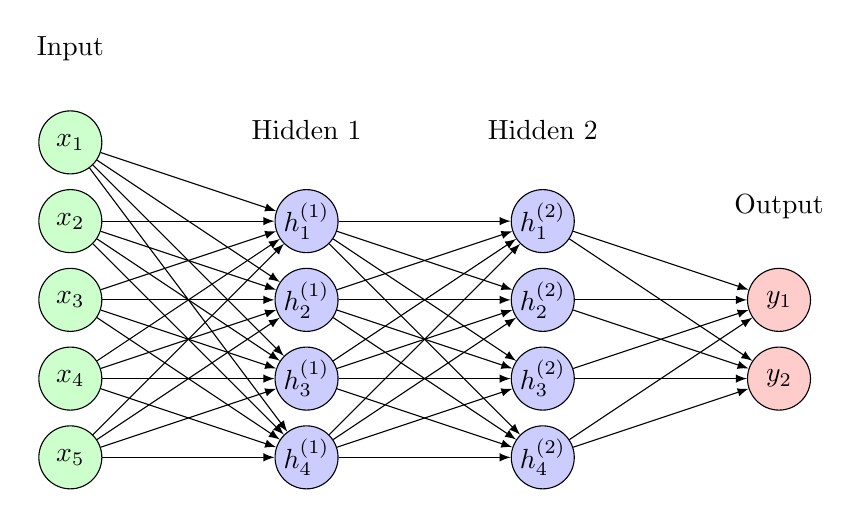
\begin{tikzpicture}[
        neuron/.style={circle, draw, minimum size=0.8cm, inner sep=0pt},
        input/.style={neuron, fill=green!20},
        hidden/.style={neuron, fill=blue!20},
        output/.style={neuron, fill=red!20},
        arrow/.style={->, >=latex}
    ]
        % Input Layer (5 Neuronen)
        \foreach \i in {1,...,5}
            \node[input] (I\i) at (0, -\i) {$x_{\i}$};

        % Hidden Layer 1 (4 Neuronen)
        \foreach \h in {1,...,4}
            \node[hidden] (H1\h) at (3, -\h - 1) {$h^{(1)}_{\h}$};

        % Hidden Layer 2 (4 Neuronen)
        \foreach \h in {1,...,4}
            \node[hidden] (H2\h) at (6, -\h - 1) {$h^{(2)}_{\h}$};

        % Output Layer (2 Neuronen)
        \foreach \o in {1,...,2}
            \node[output] (O\o) at (9, -\o - 2) {$y_{\o}$};
        
        % Labels
        \node[above=0.5cm] at (I1.north) {Input};
        \node[above=0.5cm] at (H11.north) {Hidden 1};
        \node[above=0.5cm] at (H21.north) {Hidden 2};
        \node[above=0.5cm] at (O1.north) {Output};

        % Verbindungen Input -> Hidden 1
        \foreach \i in {1,...,5}
            \foreach \h in {1,...,4}
                \draw[arrow] (I\i) -- (H1\h);

        % Verbindungen Hidden 1 -> Hidden 2
        \foreach \h in {1,...,4}
            \foreach \k in {1,...,4}
                \draw[arrow] (H1\h) -- (H2\k);

        % Verbindungen Hidden 2 -> Output
        \foreach \h in {1,...,4}
            \foreach \o in {1,...,2}
                \draw[arrow] (H2\h) -- (O\o);

    \end{tikzpicture}
    \caption{Schematische Darstellung der ursprünglichen, fully-connected Netzarchitektur.}
    \label{fig:nn_architektur_original}
\end{figure}

\begin{figure}[htbp]
    \centering
    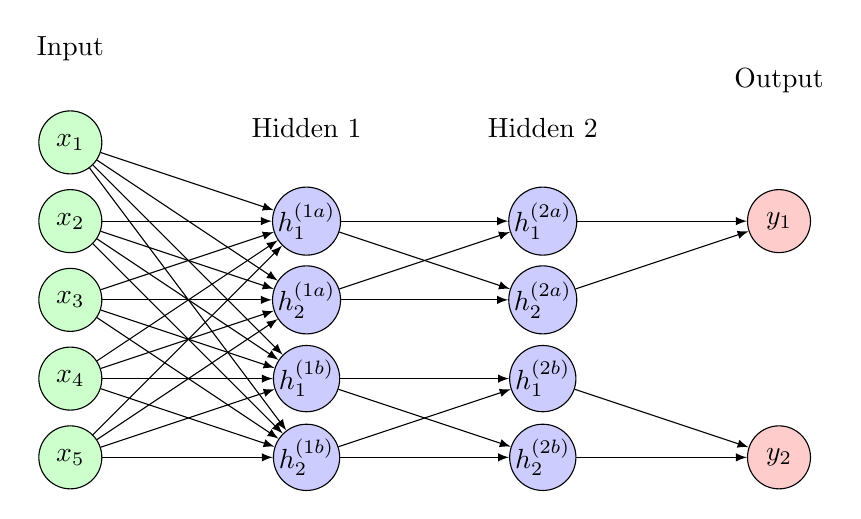
\begin{tikzpicture}[
        neuron/.style={circle, draw, minimum size=0.8cm, inner sep=0pt},
        input/.style={neuron, fill=green!20},
        hidden/.style={neuron, fill=blue!20},
        output/.style={neuron, fill=red!20},
        arrow/.style={->, >=latex}
    ]
        % Input Layer (5 Neuronen)
        \foreach \i in {1,...,5}
            \node[input] (I\i) at (0, -\i) {$x_{\i}$};

        % Hidden Layer 1 - Split (2 groups of 2)
        % Group A (Head 1)
        \foreach \h in {1,...,2}
            \node[hidden] (H1a\h) at (3, -\h - 1) {$h^{(1a)}_{\h}$};
        % Group B (Head 2)
        \foreach \h in {1,...,2}
            \node[hidden] (H1b\h) at (3, -\h - 3) {$h^{(1b)}_{\h}$};

        % Hidden Layer 2 - Split (2 groups of 2)
        % Group A (connected to y1)
        \foreach \h in {1,...,2}
            \node[hidden] (H2a\h) at (6, -\h - 1) {$h^{(2a)}_{\h}$};
        % Group B (connected to y2)
        \foreach \h in {1,...,2}
            \node[hidden] (H2b\h) at (6, -\h - 3) {$h^{(2b)}_{\h}$};

        % Output Layer (2 Neuronen)
        \node[output] (O1) at (9, -2) {$y_{1}$};
        \node[output] (O2) at (9, -5) {$y_{2}$};
        
        % Labels
        \node[above=0.5cm] at (I1.north) {Input};
        \node[above=0.5cm] at (H1a1.north) {Hidden 1};
        \node[above=0.5cm] at (H2a1.north) {Hidden 2};
        \node[above=0.5cm] at (9, -1) {Output};

        % Verbindungen Input -> Hidden 1 (A & B)
        \foreach \i in {1,...,5} {
            \foreach \k in {1,...,2} {
                \draw[arrow] (I\i) -- (H1a\k);
                \draw[arrow] (I\i) -- (H1b\k);
            }
        }

        % Verbindungen Hidden 1 A -> Hidden 2 A
        \foreach \h in {1,...,2}
            \foreach \k in {1,...,2}
                \draw[arrow] (H1a\h) -- (H2a\k);

        % Verbindungen Hidden 1 B -> Hidden 2 B
        \foreach \h in {1,...,2}
            \foreach \k in {1,...,2}
                \draw[arrow] (H1b\h) -- (H2b\k);

        % Verbindungen Hidden 2 A -> Output 1
        \foreach \h in {1,...,2}
            \draw[arrow] (H2a\h) -- (O1);

        % Verbindungen Hidden 2 B -> Output 2
        \foreach \h in {1,...,2}
            \draw[arrow] (H2b\h) -- (O2);

    \end{tikzpicture}
    \caption{Schematische Darstellung der Netzarchitektur mit vollständig getrennten Pfaden (Separate Heads) ab der Eingabeschicht.}
    \label{fig:nn_architektur_split}
\end{figure}

\begin{figure}[htbp]
    \centering
    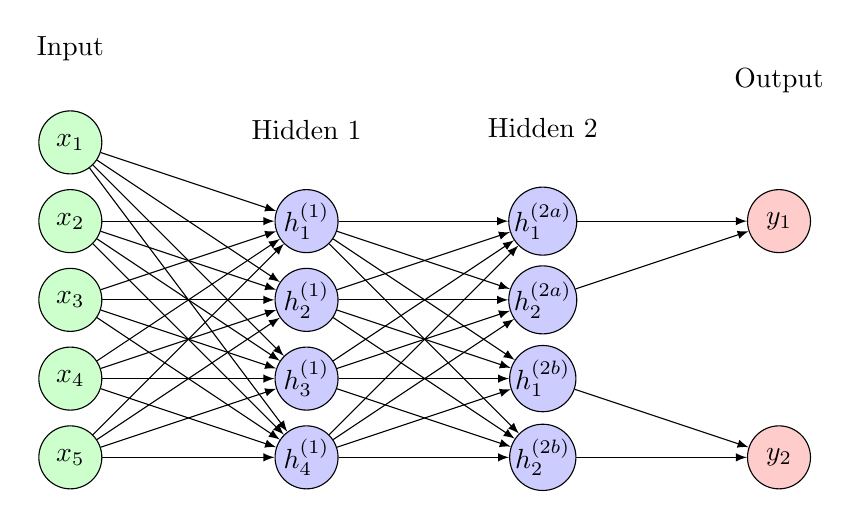
\begin{tikzpicture}[
        neuron/.style={circle, draw, minimum size=0.8cm, inner sep=0pt},
        input/.style={neuron, fill=green!20},
        hidden/.style={neuron, fill=blue!20},
        output/.style={neuron, fill=red!20},
        arrow/.style={->, >=latex}
    ]
        % Input Layer (5 Neuronen)
        \foreach \i in {1,...,5}
            \node[input] (I\i) at (0, -\i) {$x_{\i}$};

        % Hidden Layer 1 (4 Neuronen) - Shared
        \foreach \h in {1,...,4}
            \node[hidden] (H1\h) at (3, -\h - 1) {$h^{(1)}_{\h}$};

        % Hidden Layer 2 - Split (2 groups of 2)
        % Group A (Head 1)
        \foreach \h in {1,...,2}
            \node[hidden] (H2a\h) at (6, -\h - 1) {$h^{(2a)}_{\h}$};
        % Group B (Head 2)
        \foreach \h in {1,...,2}
            \node[hidden] (H2b\h) at (6, -\h - 3) {$h^{(2b)}_{\h}$};

        % Output Layer (2 Neuronen)
        \node[output] (O1) at (9, -2) {$y_{1}$};
        \node[output] (O2) at (9, -5) {$y_{2}$};
        
        % Labels
        \node[above=0.5cm] at (I1.north) {Input};
        \node[above=0.5cm] at (H11.north) {Hidden 1};
        \node[above=0.5cm] at (H2a1.north) {Hidden 2};
        \node[above=0.5cm] at (9, -1) {Output};

        % Verbindungen Input -> Hidden 1
        \foreach \i in {1,...,5}
            \foreach \h in {1,...,4}
                \draw[arrow] (I\i) -- (H1\h);

        % Verbindungen Hidden 1 -> Hidden 2 (A & B)
        \foreach \h in {1,...,4} {
            \foreach \k in {1,...,2} {
                \draw[arrow] (H1\h) -- (H2a\k);
                \draw[arrow] (H1\h) -- (H2b\k);
            }
        }

        % Verbindungen Hidden 2 A -> Output 1
        \foreach \h in {1,...,2}
            \draw[arrow] (H2a\h) -- (O1);

        % Verbindungen Hidden 2 B -> Output 2
        \foreach \h in {1,...,2}
            \draw[arrow] (H2b\h) -- (O2);

    \end{tikzpicture}
    \caption{Schematische Darstellung einer hybriden Netzarchitektur (Mischform). Die Pfade teilen sich zunächst gemeinsame Schichten (Shared Layers, hier Hidden 1), bevor sie sich trennen.}
    \label{fig:nn_architektur_hybrid}
\end{figure}

Die praktische Umsetzung dieser Architektur ist in Abbildung \ref{fig:nn_architektur_split} visualisiert, während Listing \ref{lst:branching_network} die zugehörige Implementierung zeigt. Im Gegensatz zur vollständig verbundenen Architektur in Abbildung \ref{fig:nn_architektur_original} werden hier bereits im ersten Hidden-Layer die Neuronen in funktional getrennte Gruppen unterteilt. Dieser Split zieht sich durch alle folgenden Schichten. Gruppe A verarbeitet Informationen exklusiv für den diskreten Aktionskopf ($y_1$), während Gruppe B ausschließlich den kontinuierlichen Ausgang ($y_2$) speist. Diese vollständige topologische Trennung verhindert sicher, dass der Optimierungsprozess für die Entscheidungskomponente die Repräsentationen für die Steuerungskomponente überschreibt.

